\chapter{Histogram based image enhancement}
\lecture{6}{15/11}

\begin{definition}[Histogram function]
    The \textbf{histogram function} (or \textbf{histogram distribution}) of an image is a function defined over all possible intensity levels. For each intesity level, its value is equal to the frequency of pixels with that intensity.
\end{definition}

\begin{figure}
    \centering
    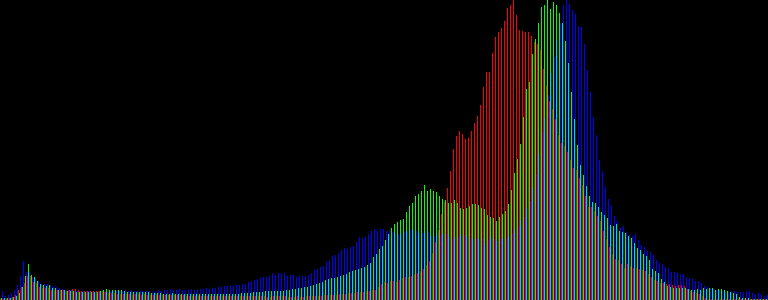
\includegraphics[width=0.8\linewidth]{images/image-histogram.png}
    \caption{An example of a image histogram showing the red, green, and blue pixel intesity frequencies.}
    \label{fig:image-histogram}
\end{figure}

\begin{algorithm}[Constructing a grayscale histogram function of an image.]
    \hspace{0em}
    \begin{algorithmic}[1]
        \Procedure{ConstructHistogram}{image $I$}
        \State initialise array histogram array entries to $0$
        \For{each pixel $I(i,j)$ within $I$}
            \State histogram(I(i,j)) = histogram(I(i, j)) + 1
        \EndFor
        \EndProcedure
    \end{algorithmic}
\end{algorithm}

\begin{remark}
    It is clear to see that more complex scenes will produce more complex pixel distributions in the histogram. 
\end{remark}

\begin{definition}[Normalisation]
    \textbf{Normalisation} (or \textbf{contrast stretching}) is the operation of stretching the pixel range over a larger dynamic range. Given $I: \R^2 \to \{ \text{min}, ..., \text{max} \}$, the \textbf{linear normalisation} of a grayscale digital image is performed according to
    \[ I_N = (I - \text{min}) \left( \frac{\text{newMax} - \text{newMin}}{\text{max} - \text{min}} \right) + \text{newMin}. \]
\end{definition}

\begin{figure}
    \centering
    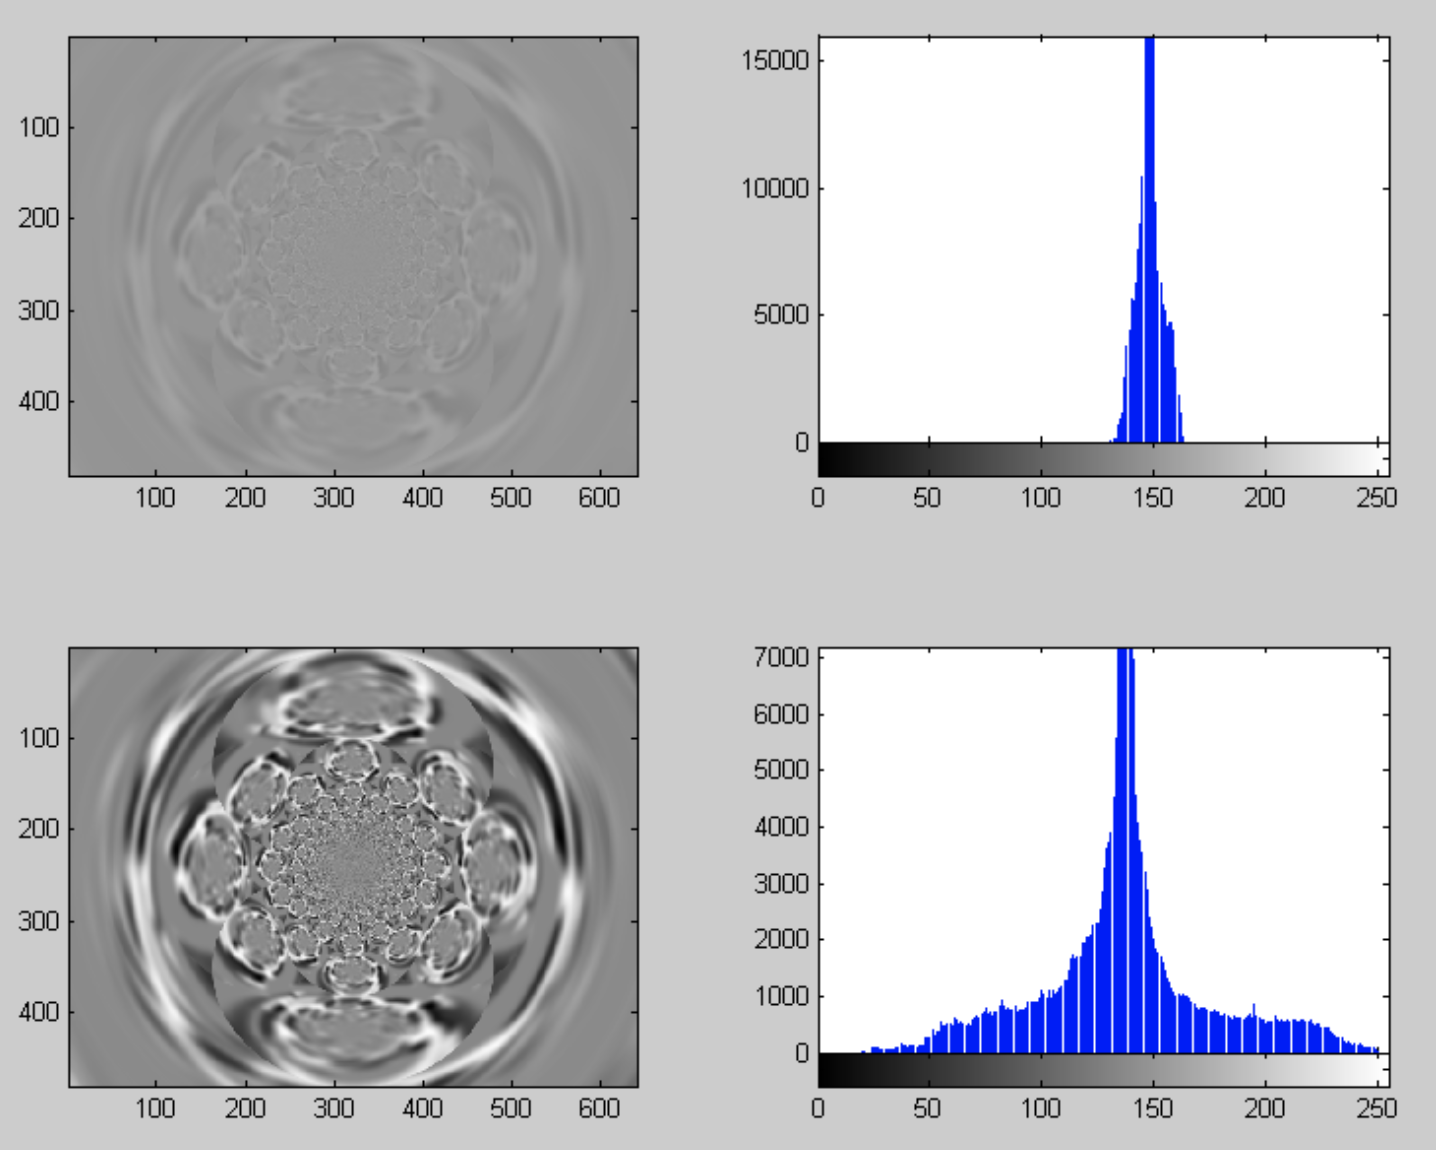
\includegraphics[width=0.8\linewidth]{images/normalisation.png}
    \caption{An example of constrast stretching with the histogram functions.}
    \label{fig:normalisation}
\end{figure}

\begin{remark}
    There may be outliers in the image (such as salt and pepper noise) which can make it possible that the new minimum and maximums are equal to the old minimum and maximums. This results in no effect on the image. Here are two solutions to dealing with outliers:
    \begin{enumerate}
        \item select the minimum and maximum as the 5th and 95th percentile (or any percentiles), and take the new minimum and maximum as the minimum and maximum possible intensity level, if any intensity values are mapped outside of this range just set it to the limit; and
        \item find the modal intensity value and set a cut-off as a percentage of this peak, if intensity values map outside of the boundary then set them to the boundary.
    \end{enumerate}
    It is clear to see that (ii) is weak for complex peaks with multiple peaks. 
\end{remark}

\begin{figure}
    \centering
    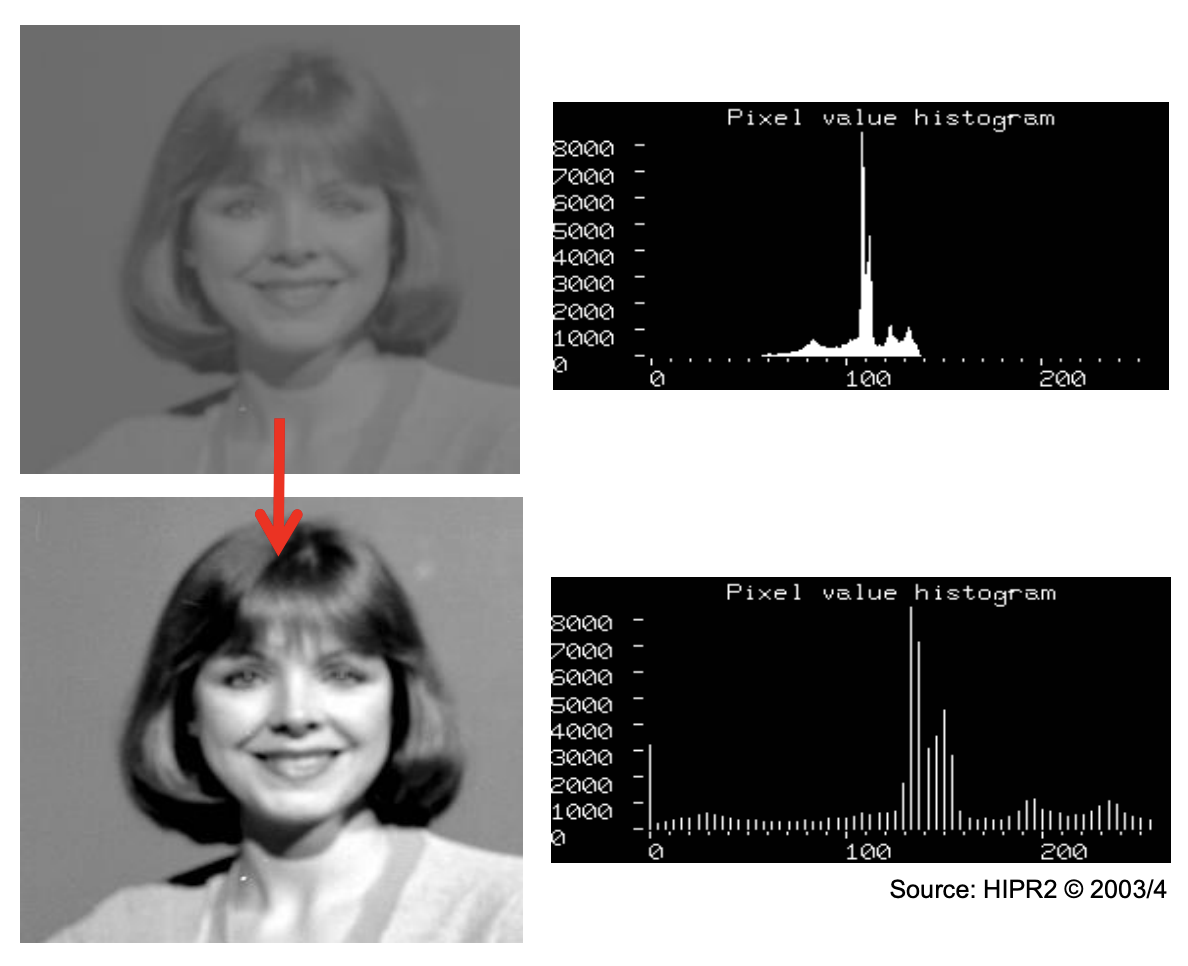
\includegraphics[width=0.8\linewidth]{images/mode-cutoff.png}
    \caption{An example of mode percentage cut-off (method (ii)) with a cut-off fraction of $0.03$.}
    \label{fig:mode-cutoff}
\end{figure}

\begin{figure}
    \centering
    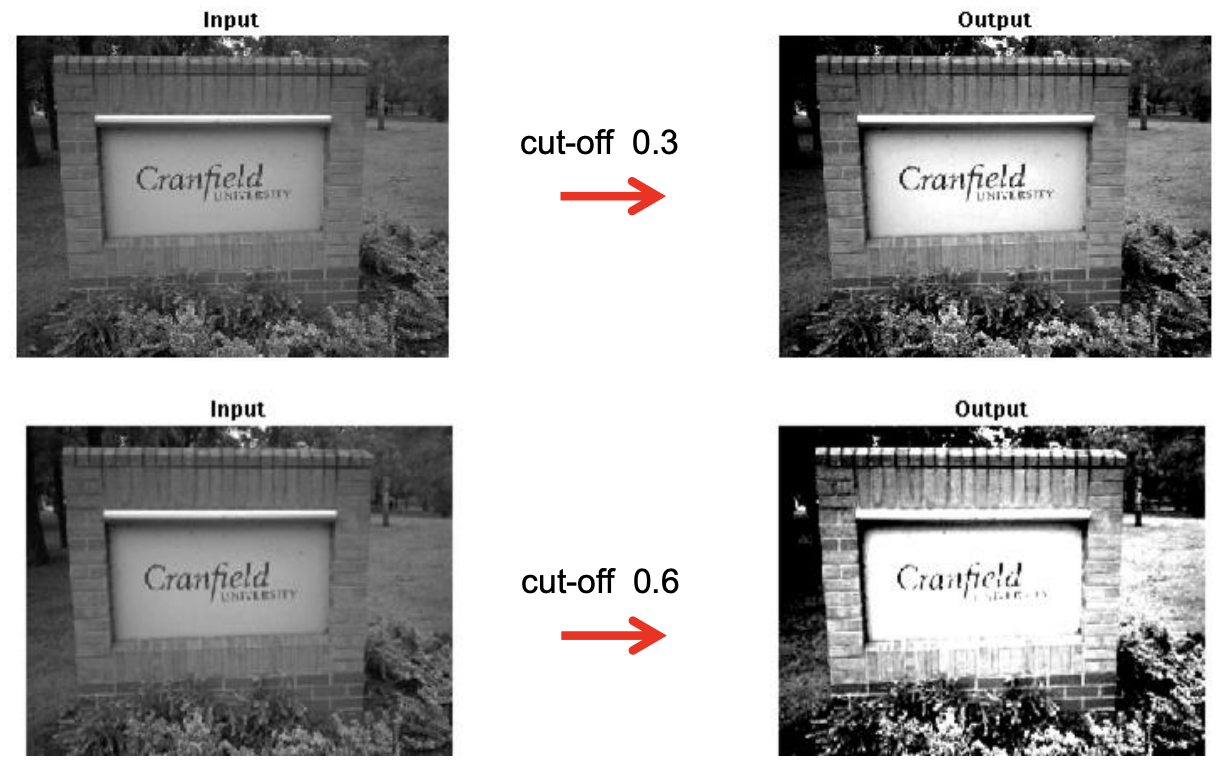
\includegraphics[width=0.8\linewidth]{images/mode-cutoff-2.png}
    \caption{A comparison of mode percentage cut-off (method (ii) with different cut-off fractions.}
    \label{fig:mode-cutoff-2}
\end{figure}

\begin{definition}[Histogram modelling]
    \textbf{Histogram modelling} is the process of modifying an image so that its histogram conforms to given conditions.
\end{definition}

\begin{definition}[Histogram equalisation]
    A type of histogram modelling, \textbf{histogram equalisation} aims to produce an output image with a uniform histogram distribution. 
\end{definition}

\begin{definition}[Cumulative histogram function]
    From a histogram function $h(i)$, we construct the \textbf{cumulative histogram function}
    \[ C(i) = \sum_{j = 1}^i h(j). \]
\end{definition}

\begin{proposition}[]
    Any given cumulative histogram function $C(i)$ is monotone increasing. 
\end{proposition}

\begin{definition}[Ideally equalised]
    Let $h(i)$ be a histogram function of an image with dynamic range $L$ made up of $N$ pixels. We say $I$ is \textbf{ideally equalised} if all intensity values appear with the same frequency. That is, $h(i) = \frac{N}{L}$. The cumulative function is then defined by
    \[ C(i) = \frac{iN}L. \]
\end{definition}

\begin{definition}[Histogram equalisation]
    A type of histogram modelling, \textbf{histogram equalisation} aims to produce an output image with a uniform histogram distribution. Histogram equalisation corresponds to the intensity transformation
    \[ t(i) = \frac LN \cdot C(i) \]
    where $C$ is the input histogram function. 
\end{definition}

\begin{example}
    Consider a single-channel image $I$ with histogram function $C(i)$, dynamic range $L = 100$, and $N$ pixels. Now let $C(50) = 0.8N$, that is, 80\% of the pixels have a value of $50$ or lower. Now let us consider the image produced via histogram equalisation $I'$ and its histogram function $C'$. Then we have
    \[ C'(50) = \frac LN \cdot C(50) = \frac {100}N \cdot 0.8N = 80. \]
\end{example}
